\begin{enumerate}[label=\thesubsection.\arabic*,ref=\thesubsection.\theenumi]
	\item 		Find the values of x and y so that the vectors
$2\hat{i}+3\hat{j}$
and 
$x\hat{i}+y\hat{j}$
are equal.
\\
\solution
From the given informatin, 
\begin{align}
	\myvec{2\\3} = \myvec{x \\ y} 
	\\
	\implies x = 2, y = 3
\end{align}

\item Find the values of $x,y,z$ so that the vectors 
$x\hat{i}+2\hat{j}+z\hat{k}$
and 
$2\hat{i}+y\hat{j}+\hat{k}$
are equal.
\item Find the sum of the vectors $\vec{a}=\hat{i}-2\hat{j}+\hat{k}$, $\vec{b}=-2\hat{i}+4\hat{j}+5\hat{k}$ and $\vec{c}=\hat{i}-6\hat{j}-7\hat{k}$.
\item Find the slope of a line, which passes through the origin and the mid point of the line segment joining the points $\vec{P}$(0,-4) and $\vec{B}$(8,0).
\label{chapters/11/10/1/5}
	\\
	\solution
The mid point of $PB$ is
\begin{align}
\vec{M} =\frac{1}{2}(\vec{P}+\vec{B})
	= \myvec{4 \\ -2}  
\end{align}
which, from  \eqref{eq:dir-vec}, is equal to the direction vector of $OM$, where $\vec{O}$ is the origin.
\begin{align}
\because \vec{M} \equiv
	 \myvec{1 \\ -\frac{1}{2}},
	m = -\frac{1}{2}
\end{align}
which, from \eqref{eq:dir-vec},  is the desired slope.
See 
		\figref{fig:11/10/1/5}.
	\begin{figure}[H]
		\centering
 %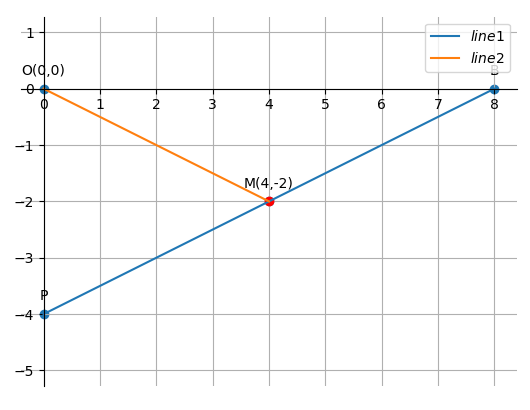
\includegraphics[width=0.75\columnwidth]{chapters/11/10/1/5/figs/line.png}
 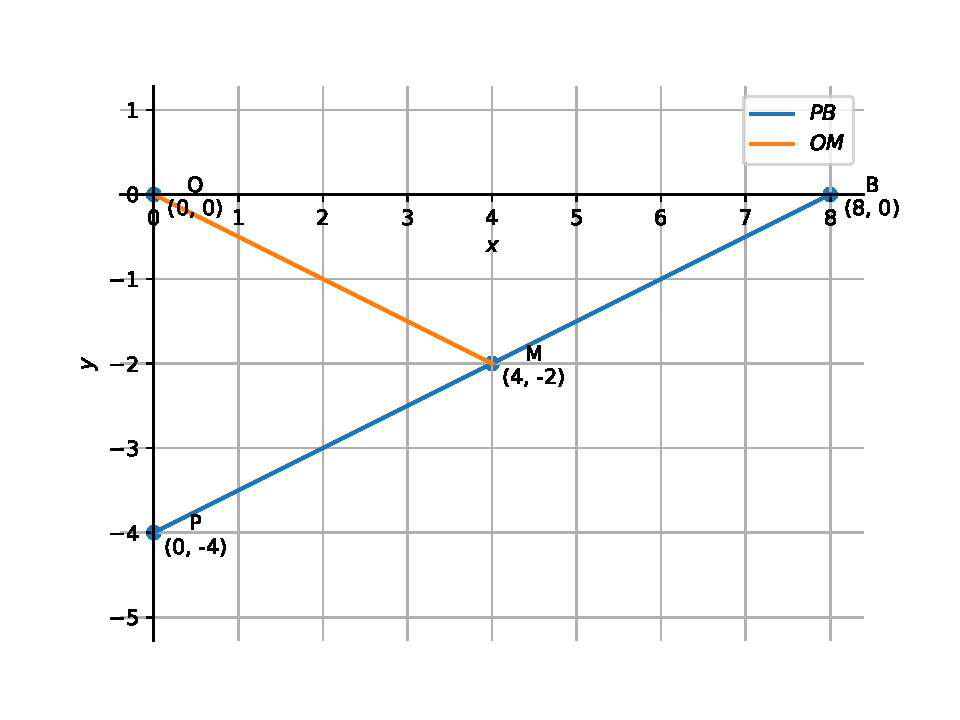
\includegraphics[width=0.75\columnwidth]{chapters/11/10/1/5/figs/fig.pdf}
		\caption{}
		\label{fig:11/10/1/5}
  	\end{figure}

\item Find the angle between x-axis and the line joining points (3,-1) and (4,-2).
\label{chapters/11/10/1/10}
\\
\solution 
The direction vector of the given line is 
\begin{align}
	\vec{C}
=\myvec{ -1\\ 1 }
\end{align}
Hence, the desired angle is given by
\begin{align}
	\cos\theta=\frac{\vec{C}^{\top}\vec{e}_1}{\norm{\vec{C}}\norm{\vec{e}_1}}
	&= -\frac{1}{\sqrt{2}}
	\\
	\implies 
	\theta&=135\degree
 \end{align}

\item A line passes through $A(x_1,y_1)$ and $B(h,k)$. If slope of the line is m, show that $(k-y_1)=m(h-x_1)$.
\label{chapters/11/10/1/12}
\\
\solution 
The direction vector
\begin{align}
	\vec{B}-\vec{A}
	=
	\myvec{
  h-x_1\\
  k-y_1
  }
   \equiv
	\myvec{
1\\
	\frac{ k-y_1}{h-x_1}
  }
  \\
	\implies m = 
	\frac{ k-y_1}{h-x_1},
\end{align}
yielding the desired result.

\item
Show that the line through the points \brak{4,7,8},\brak{2,3,4} is parallel to the line through the points \brak{-1,-2,1},\brak{1,2,5}.
	\label{12.11.2.3}
\\
\solution
	Show that the line through the points \brak{4,7,8},\brak{2,3,4} is parallel to the line through the points\brak{-1,-2,1},\brak{1,2,5}.

\textbf{Solution :}
For line passing through \brak{4,7,8},\brak{2,3,4},the direction vector,\begin{align}
    \vec{m_1}&=\myvec{-2\\-4\\-4}
\end{align}
For line passing through \brak{-1,-2,1},\brak{1,2,5},the direction vector,\begin{align}
    \vec{m_2}&=\myvec{2\\4\\4}
\end{align}
Therefore,the lines are parallel to each other.

\item The vector having intial and terminal points as (-2,5,0) and (3,7,4),respectively is
	\begin{enumerate}
\item -$\hat{i}+12\hat{j}+4\hat{k}$
\item $5\hat{i}+2\hat{j}-4\hat{k}$
\item $5\hat{i}+2\hat{j}+4\hat{k}$
\item $\hat{i}+\hat{j}+\hat{k}$
\end{enumerate}
\solution
The desired vector is
\begin{align}
	\myvec{3 \\ 7 \\ 4}
	-\myvec{-2 \\ 5 \\ 0} = 
	\myvec{5 \\ 2 \\ 4}  
\end{align}
\item Find the vector joining the points $P\brak{2,3,0}$ and $Q\brak{-1,-2,-4}$ directed from $P$ to $Q$.
\item Without using distance formula, show that points $A(– 2, – 1), B(4, 0), C(3, 3)$ and $D(–3, 2)$ are the vertices of a parallelogram.
\label{chapters/11/10/1/9}
\\
\solution
	  From \eqref{eq:two-pgm},
\begin{align}
\vec{A}-\vec{B} = 
\vec{D}-\vec{C} =  \myvec{-6\\-1}
\end{align}
Hence, $ABCD$ is a parallelogram.
See \figref{fig:chapters/11/10/1/91}.
\begin{figure}[h!]
  \centering
   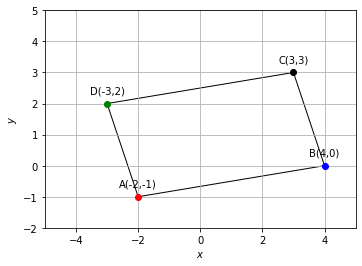
\includegraphics[width=\columnwidth]{chapters/11/10/1/9/figs/paralellogram.png}
    \caption{}
     \label{fig:chapters/11/10/1/91}  
\end{figure}




\item If the points $A(6, 1), B(8, 2), C(9, 4)$ and $D(p, 3)$ are the vertices of a parallelogram, taken in order, find the value of $p$.
\label{10/7/0/10}
\item 
If $(1, 2), (4, y), (x, 6)$ and $(3, 5)$ are the vertices of a parallelogram taken in order, find $x$ and $y$.
\label{10/7/2/6}
	\\
		\solution
	Since $ABCD$ is a parallellogram,
\begin{align}
  \label{eq:chapters/10/7/2/6/tables/det2f}
 \myvec{4 \\y } - \myvec{1 \\2 }  
= \myvec{x \\6 } - \myvec{3 \\5 }  
\\
\implies	\myvec{3\\y-2}=\myvec{x-3\\1}\\
	\text{ or, }x=6 ,y=3.
\end{align}
See  \figref{fig:chapters/10/7/2/6/Fig3}.
\begin{figure}[h!]
	\begin{center}
  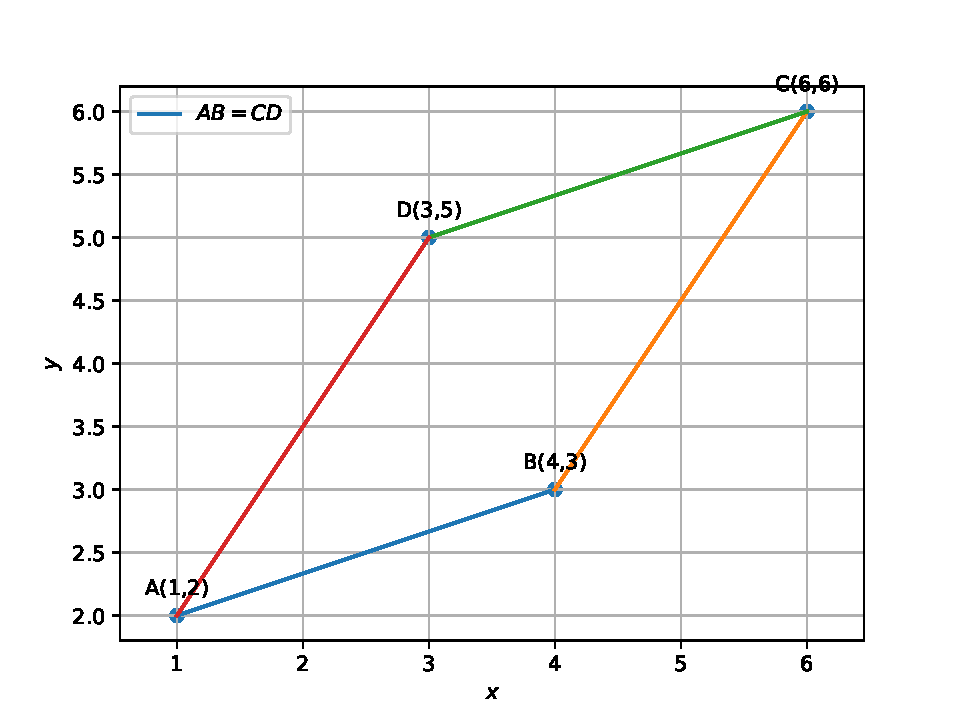
\includegraphics[width=\columnwidth]{chapters/10/7/2/6/figs/para.pdf}
	\end{center}
\caption{}
\label{fig:chapters/10/7/2/6/Fig3}
\end{figure}


\item The fourth vertex $\vec{D}$ of a parallelogram $\vec{ABCD}$ whose three vertices are
	$\vec{A} (–2, 3), \vec{B} (6, 7)\text { and } \vec{C} (8, 3)$ is
\begin{enumerate}
	\item $(0, 1)$
	\item $(0, –1)$
	\item $ (–1,0)$
	\item$(1, 0)$
\end{enumerate}
\item Verify if the points $\vec{A}(4,3), \vec{B}(6,4),\vec{C}(5,-6)$  and  $\vec{D}(-3,5)$ are the vertices of a parallelogram.
\item A girl walks 4 km towards west, then she walks 3 km in a direction 30$^{\circ}$ east of north and stops. Determine the girl's displacement from her initial point of departure.\\
	\solution
		See  
\figref{fig:chapters/12/10/5/3Fig1}.
Let the initial position
be
\begin{align}
	\vec{A}=\myvec{0\\0}
\end{align}
After going west, the position becomes
\begin{align}
			\vec{B}=\myvec{-4\\0}
\end{align}
If the final position be $\vec{C}$, from the given information,
\begin{align}
	 \vec{C}-\vec{B}=3\myvec{\cos{60\degree}\\\sin{60\degree}}
	 \implies 
	\vec{C}  
=\myvec{\frac{-5}{2}\\[2pt] \frac{3\sqrt{3}}{2}}
\end{align}
which is the desired displacement. 
\begin{figure}[H] 
 \begin{center} 
 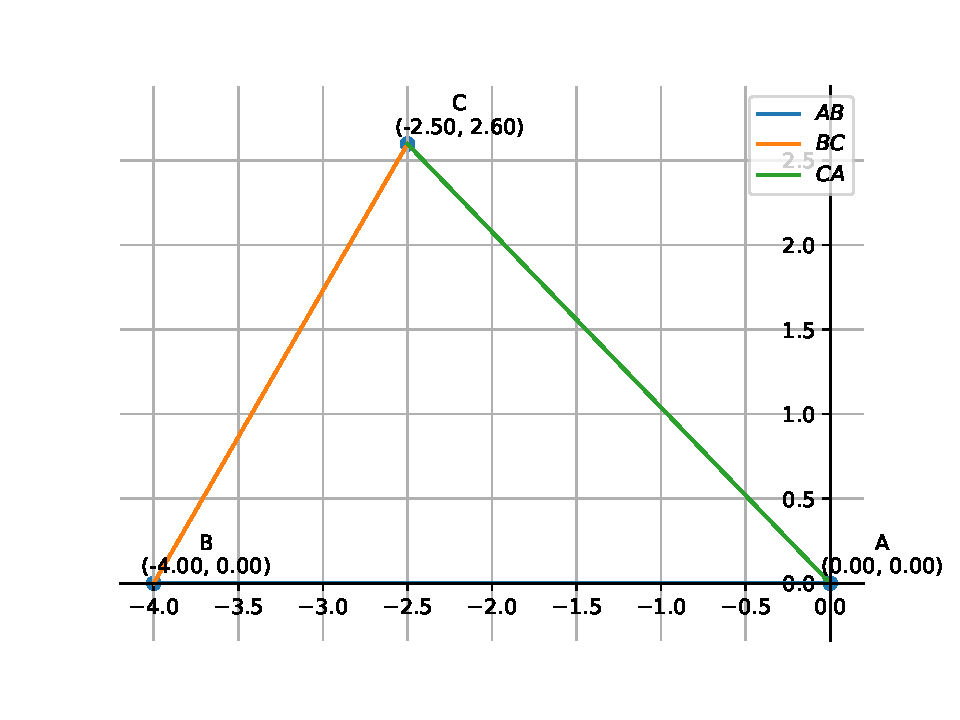
\includegraphics[width=0.75\columnwidth]{chapters/12/10/5/3/figs/fig.pdf} 
 \end{center} 
\caption{} 
\label{fig:chapters/12/10/5/3Fig1} 
\end{figure}

\end{enumerate}
